\documentclass{article}
\usepackage[x11names, rgb]{xcolor}
\usepackage[utf8]{inputenc}
\usepackage{tikz}
\usetikzlibrary{snakes,arrows,shapes}
\usepackage{amsmath}
%
%

%

%

\begin{document}
\pagestyle{empty}
%
%
%

\enlargethispage{100cm}
% Start of code
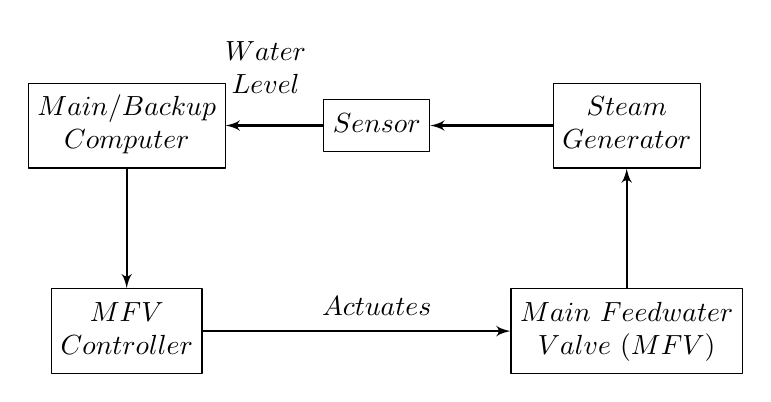
\begin{tikzpicture}[>=latex',line join=bevel,]
%%
\node (1) at (27bp,92bp) [draw,rectangle] {$\begin{matrix} Main/Backup \\ Computer  \end{matrix}$};
  \node (3) at (207bp,92bp) [draw,rectangle] {$\begin{matrix} Steam \\ Generator \end{matrix}$};
  \node (2) at (117bp,92bp) [draw,rectangle] {$\begin{matrix} Sensor \end{matrix}$};
  \node (5) at (207bp,18bp) [draw,rectangle] {$\begin{matrix} Main \text{ } Feedwater \\ Valve \text{ } (MFV) \end{matrix}$};
  \node (4) at (27bp,18bp) [draw,rectangle] {$\begin{matrix} MFV \\ Controller \end{matrix}$};
  \draw [->,thick] (5) ..controls (207bp,44.387bp) and (207bp,54.431bp)  .. (3);
  \draw [<-,thick] (2) ..controls (162.76bp,92bp) and (171.36bp,92bp)  .. (3);
  \draw [->,thick] (1) ..controls (27bp,65.464bp) and (27bp,55.538bp)  .. (4);
  \draw [->,thick] (4) ..controls (85.177bp,18bp) and (135.5bp,18bp)  .. (5);
  \definecolor{strokecol}{rgb}{0.0,0.0,0.0};
  \pgfsetstrokecolor{strokecol}
  \draw (117bp,26bp) node {$\begin{matrix} Actuates \end{matrix}$};
  \draw [<-,thick] (1) ..controls (72.713bp,92bp) and (81.658bp,92bp)  .. (2);
  \draw (72bp,100bp) node {$\begin{matrix} & Water \\ & Level \\ &  \\ & \end{matrix}$};
%
\end{tikzpicture}
% End of code

%
\end{document}
%



